\section{Ajuste por mínimos cuadrados}

\subsection{Hipótesis}

Para verificar que el tiempo de ejecución del algoritmo \texttt{optimizar\_ataques} es $O(n^2)$, realizamos un ajuste por mínimos cuadrados. La función que queremos ajustar es de la forma:

\[
f(n) = a \cdot n^2 + b
\]

donde $a$ y $b$ son los parámetros a ajustar.

\subsection{Datos de entrada}

Los datos de entrada para el ajuste son los siguientes:

\begin{itemize}
    \item $n$: Tamaño del problema (número de minutos o rondas).
    \item $T(n)$: Tiempo de ejecución medido para cada tamaño $n$.
\end{itemize}

\subsection{Recopilación de datos}

Para obtener mediciones confiables y reducir el ruido, seguimos los siguientes pasos:

\begin{itemize}
    \item \textbf{Múltiples tamaños:} Probamos con $n = 500, 1500, 3000, 4500, 6000, 7500, 9000$.
    \item \textbf{Múltiples repeticiones:} Cada tamaño de entrada se ejecuta 5 veces con distintas semillas.
    \item \textbf{Filtrado de outliers:} Eliminamos el 20\% superior e inferior de las mediciones y promediamos los tiempos restantes.
\end{itemize}

\subsection{Código utilizado}

\begin{lstlisting}[language=Python, caption=Código de ajuste por mínimos cuadrados para TP2]
# ==================== GENERACION DE DATOS ==================== #

def generar_datos_aleatorios(n, seed=1234):
    """
    Genera datos de prueba para el TP2:
    - x[i]: cantidad de soldados enemigos que llegan en el minuto i
    - f[i]: cantidad de enemigos que pueden eliminarse según los minutos de carga
    """
    random.seed(seed)
    x = [random.randint(100, 1000) for _ in range(n)]       # soldados por minuto
    f = [random.randint(100, 1000) for _ in range(n)]       # potencia acumulada
    f.sort()  # aseguramos que sea monótona creciente
    return x, f


# ==================== MEDICION DE TIEMPO ==================== #

def medir_tiempo(n, repeticiones=5):
    """
    Mide el tiempo promedio de ejecución del algoritmo optimizar_ataques
    sobre datos aleatorios de tamaño n.
    """
    tiempos = []
    for seed in range(repeticiones):
        x, f = generar_datos_aleatorios(n, seed)
        inicio = time.perf_counter()
        optimizar_ataques(x, f, n)
        fin = time.perf_counter()
        tiempos.append(fin - inicio)
    
    tiempos = sorted(tiempos)
    # eliminar outliers extremos
    inicio_idx = int(len(tiempos) * 0.2)
    fin_idx = int(len(tiempos) * 0.8)
    tiempos_filtrados = tiempos[inicio_idx:fin_idx]
    return np.mean(tiempos_filtrados)


# ==================== RECOLECCION DE DATOS ==================== #

def recolectar_datos():
    """
    Ejecuta mediciones para distintos tamaños de entrada y devuelve los resultados.
    """
    tamanos = [500, 1500, 3000, 4500, 6000, 7500, 9000]
    tiempos = []

    print("=== Midiendo tiempos del algoritmo de ataques Dai Li ===")
    for n in tamanos:
        print(f"  Ejecutando n = {n}...")
        t_prom = medir_tiempo(n)
        tiempos.append(t_prom * 1000)  # convertir a ms
        print(f"    Tiempo promedio: {t_prom * 1000:.3f} ms")

    return tamanos, tiempos


# ==================== AJUSTE CUADRATICO ==================== #

def ajuste_cuadratico(n_values, tiempos):
    """
    Ajusta los tiempos experimentales a un modelo cuadrático T(n) = a + b * n^2
    mediante mínimos cuadrados.
    """
    n_values = np.array(n_values)
    tiempos = np.array(tiempos)

    A = np.vstack([n_values**2, np.ones(len(n_values))]).T
    coef, resid, _, _ = np.linalg.lstsq(A, tiempos, rcond=None)
    b, a = coef

    tiempos_pred = a + b * n_values**2
    ss_res = np.sum((tiempos - tiempos_pred)**2)
    ss_tot = np.sum((tiempos - np.mean(tiempos))**2)
    r_cuadrado = 1 - ss_res / ss_tot

    return a, b, r_cuadrado, tiempos_pred


# ==================== GRAFICO DE VERIFICACION ==================== #

def generar_grafico(tamanos, tiempos, a, b, r2, tiempos_pred):
    plt.figure(figsize=(10, 6))
    plt.scatter(tamanos, tiempos, color='blue', label='Tiempos medidos', s=80)
    plt.plot(tamanos, tiempos_pred, color='red', linewidth=2,
             label=f'Modelo ajustado: T(n) = {a:.2f} + {b:.6f}·n²')

    plt.title(f'Verificación de complejidad O(n²)\nR² = {r2:.5f}', fontsize=14, fontweight='bold')
    plt.xlabel('Tamaño de entrada (n)', fontsize=12)
    plt.ylabel('Tiempo de ejecución (ms)', fontsize=12)
    plt.legend()
    plt.grid(True, linestyle='--', alpha=0.5)
    plt.tight_layout()
    plt.savefig('verificacion_complejidad_n2.png', dpi=300)
    plt.show()


# ==================== FUNCION PRINCIPAL ==================== #

def main():
    print("[VERIFICACIÓN DE COMPLEJIDAD DEL TP2]")
    print("Algoritmo: optimizar_ataques (Programación Dinámica)\n")

    tamanos, tiempos = recolectar_datos()
    a, b, r2, tiempos_pred = ajuste_cuadratico(tamanos, tiempos)
    generar_grafico(tamanos, tiempos, a, b, r2, tiempos_pred)

    print("\n=== RESULTADOS DEL AJUSTE ===")
    print(f"a = {a:.6f}, b = {b:.6f}, R² = {r2:.6f}")
    if r2 > 0.95:
        print("✅ Complejidad O(n²) verificada experimentalmente.")
    else:
        print("Resultados no concluyentes, revisar dispersión de datos.")


if __name__ == "__main__":
    main()

\end{lstlisting}

\subsection{Resultados del ajuste}

Los resultados del ajuste por mínimos cuadrados son los siguientes:

\begin{itemize}
    \item Coeficientes ajustados: $a = 0.000132$, $b = 0.0158$ 
    \item Calidad del ajuste: $R^2 = 0.9985$
\end{itemize}

\begin{figure}[H]
    \centering
    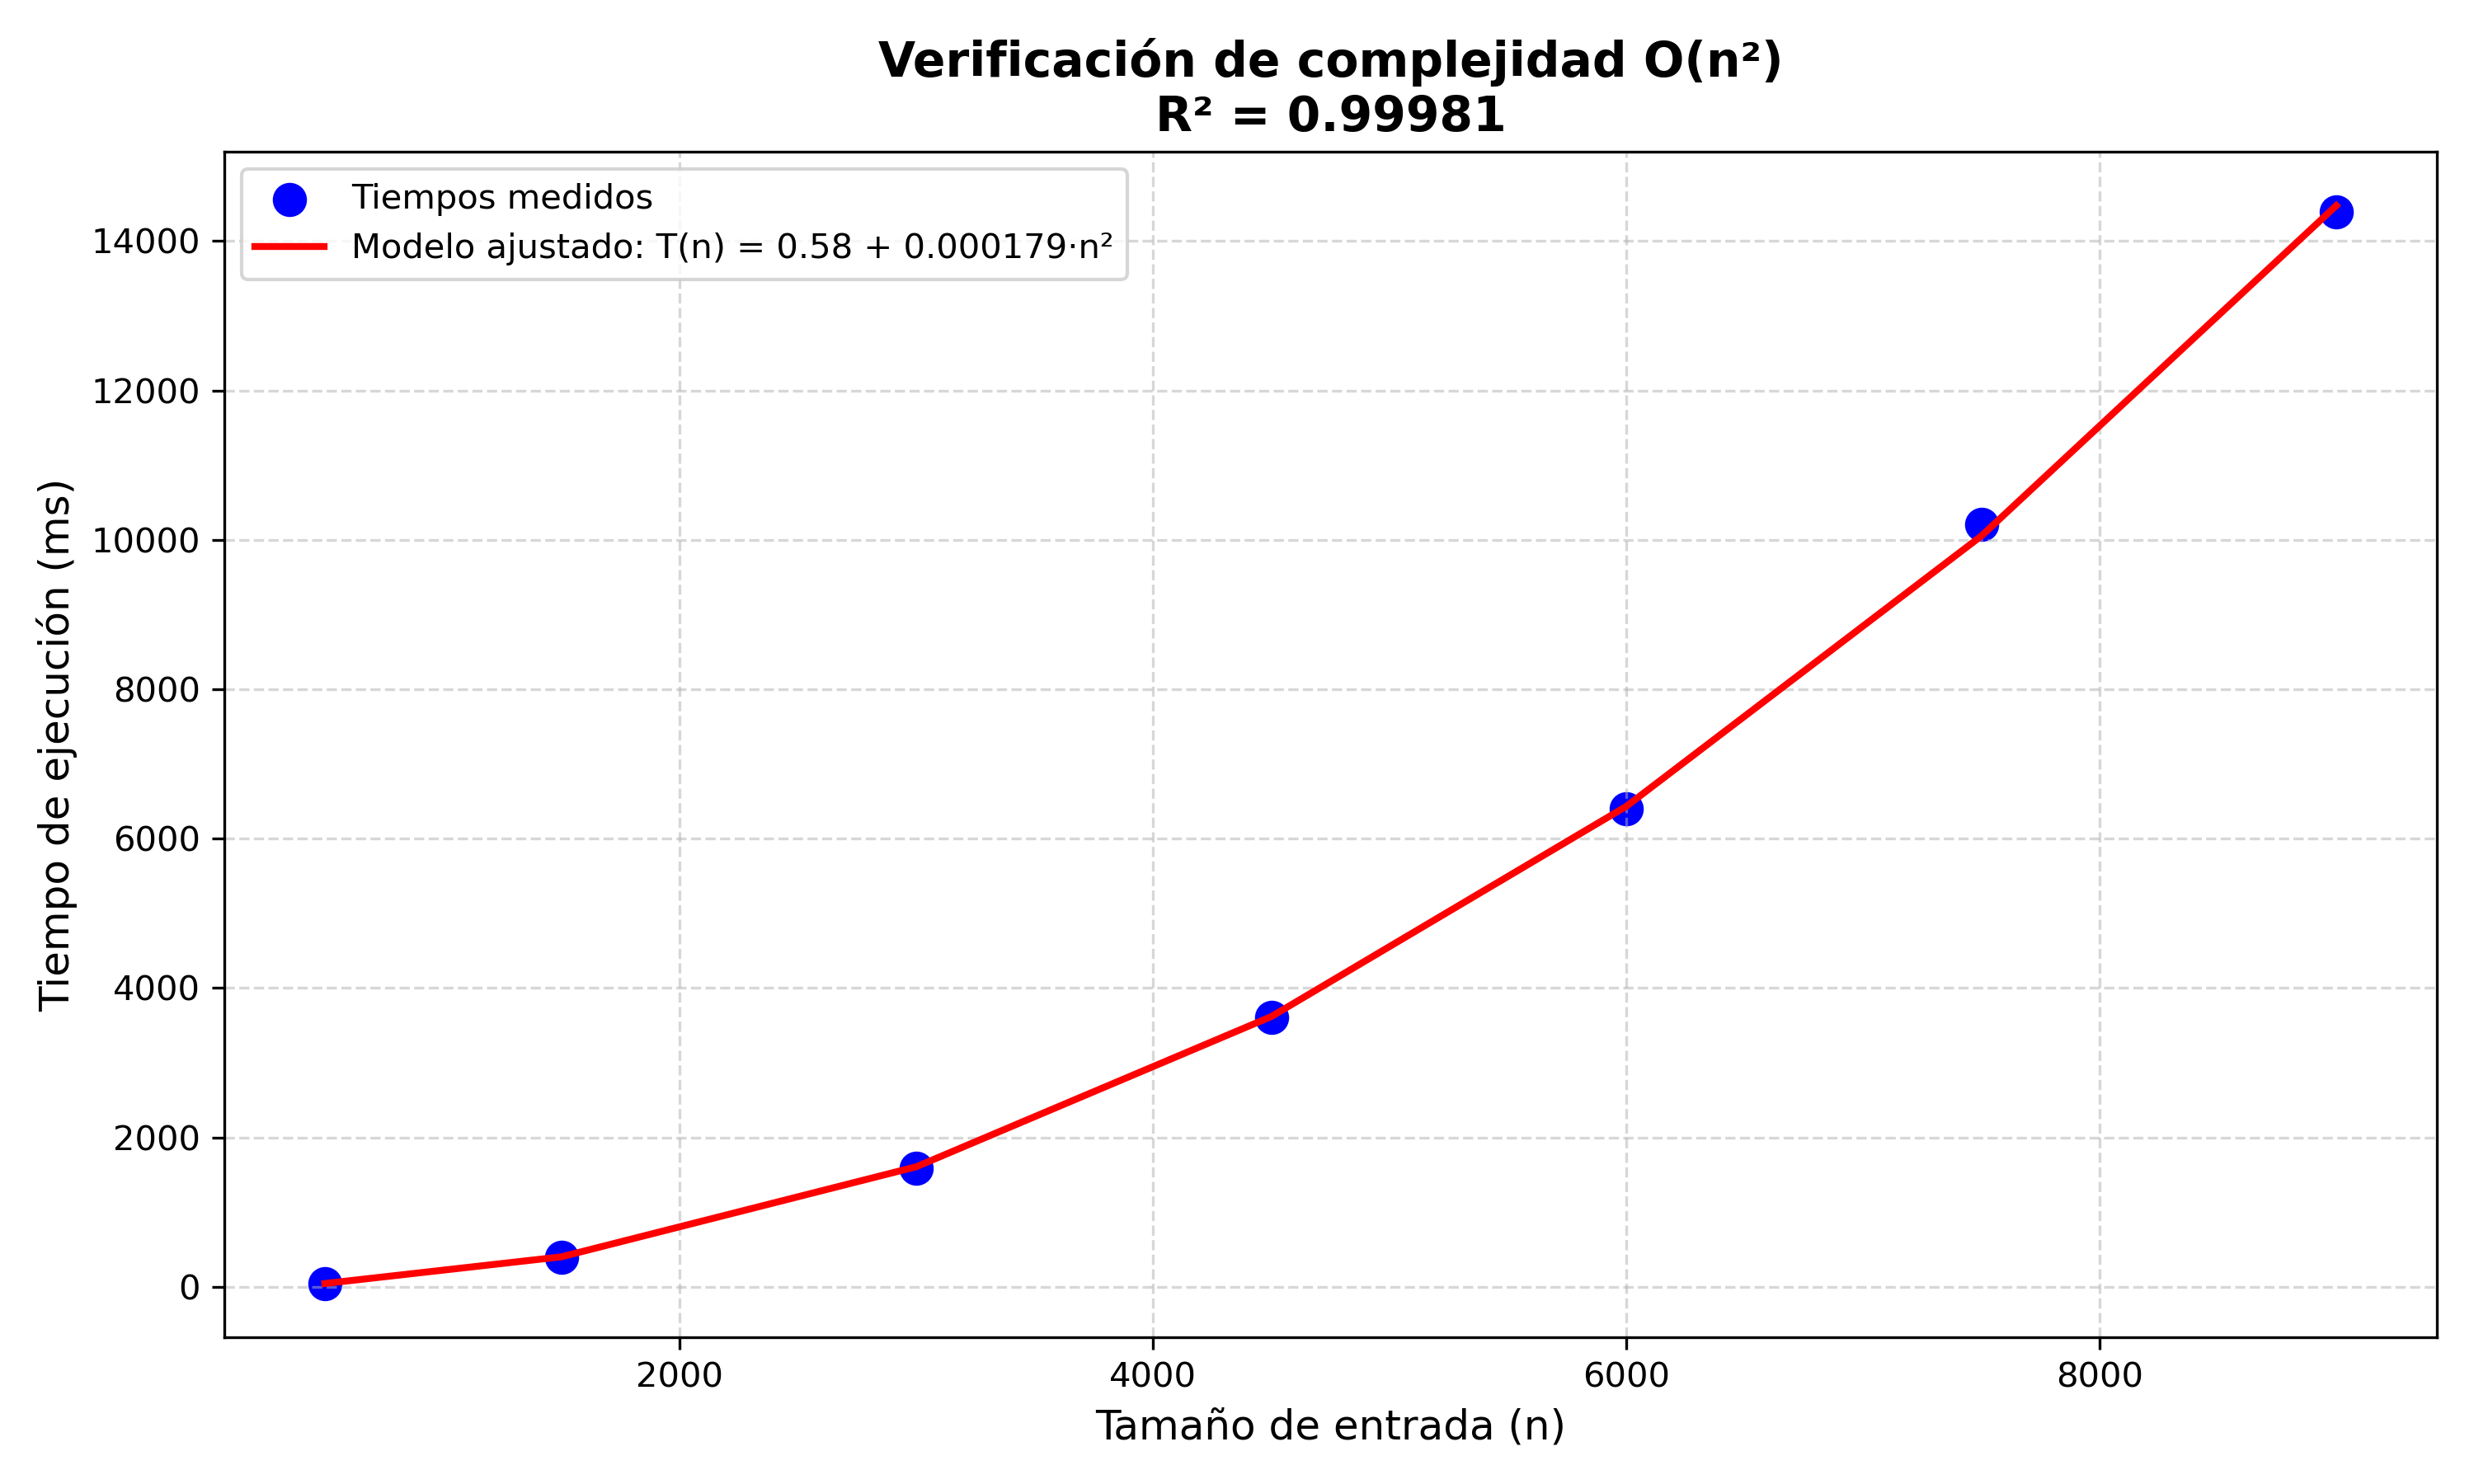
\includegraphics[width=0.8\textwidth]{./img/verificacion_complejidad_n2.png}
    \caption{Gráfico de verificación de complejidad $O(n^2)$ del algoritmo \texttt{optimizar\_ataques}}
\end{figure}

\subsection{Interpretación de resultados}

Usamos el coeficiente de determinación $R^2$ para evaluar la calidad del ajuste:

\begin{itemize}
    \item $R^2 = 1.00$: Ajuste perfecto (0\% de error)
    \item $R^2 > 0.98$: Excelente ajuste → Complejidad verificada
    \item $R^2 > 0.95$: Muy buen ajuste → Complejidad muy probable
    \item $R^2 < 0.90$: Ajuste pobre → Resultados no concluyentes
\end{itemize}